\chapter{Results and Discussion}
\label{cha:result}
In this section we present a simplified synthetic computer network developed in Python, validation of the models correctness with respect to assumptions regarding queue length stabilization can be found in appendix B. Once validated we apply baseline techniques introduced in \cref{cha:methodology} to test our new methods for nefarious router identification. We compared these results to previous analytical techniques, highlighting trade-offs in accuracy for generally applicability, deploy-ability and run time within \cref{sec:Rnefarouterdetection}. During this analysis several interesting behaviours were encountered in edge cases, these findings are shown and further experiments conducted on hypothesised explanations for the behaviour within \cref{sec:Asympathicpdv} and \cref{ssec:Rmetricnormalisation}. Of particular noteworthiness is that the investigation into unexpectedly poor inferential results from router level \pdv  behaviour in \cref{ssec:Rmetricnormalisation} revealed a flaw within previous work's inferential calculation, necessitating changes to the experimental methodology. We then move to testing the impacts of optimal probe allocation techniques on our inferential accuracy in \cref{sec:Rprobingoptimality}, ...\par
\todo{Very brief outline of accuracy changes based on A/D optimality, (it went up/down by x)}
Finally we construct a simulated network using real world topological and traffic data-sets within the NS3 framework to test our new method's performance in real world networks, formulating a quantitative response to our project's overarching goal.

\section{Nefarious Router Detection}
\label{sec:Rnefarouterdetection}

\subsection{Packet Delay Inference Validity}
To test our core hypothesis that packet delay metrics are a valid indicator of nefarious packet delaying router behaviour we consider a baseline 6 router network from \cref{sec:Mnetworkprobing} shown in \cref{fig:M6routertop}. To observe the impact of nefarious behaviour on packet delay six experiments were conducted with each router $r_0,\dots, r_5$ designed as nefarious in each experiment respectively. Each experiment consisted of 50 trials over range of holding probabilities for the nefarious router between 0 and 1, in each trial average packet delay statistics from 50 simulations were collected from each router every timestep post queue stabilization. Plots of router packet delay average (PDA) and variation (PDV) are shown in \cref{fig:Rvarnefrouter}.\par
Initially all nefarious router packet delay metrics were grouped together in the analysis but as shown in \cref{tbl:MrouterPDAvars} large variances in PDA, and consequently PDV, were observed in delay probabilities 0.2 - 0.5. Closer investigation revealed that this discrepancy of variances was between 3 groups of routers: $\{r_0,\ r_5\}$, $\{r_1,\ r_4\}$, and $\{r_2,\ r_3\}$ this grouping is validated by the table of variances in \cref{tab:Rallvars}. From this we find that the intra-group variance is 100.60, 34.46, and 179.92 for each groups respectively however they have an average inter-group variance of 862.99. Each group has a common feature, that its comprising routers are indistinguishable via their values in the adjacency matrix. We investigate of the cause and impacts of this symmetry in \cref{sec:Asympathicpdv}.\par
Using these grouping its clear that the nefarious router's PDA differs significantly from all other routers in the network, with a hold probability of 0.5 resulting in a router PDA $\approx$3232 times larger than that of the 2nd largest PDA. Of interest is the behaviour of $r_0$ and $r_5$ when nefarious as although these routers connect to half as many routers as the others their nefarious behaviour can still be inferred through PDA.\par

\begin{figure}[H]
    \centering
    \tikzsetnextfilename{6routerpdvtopology}
    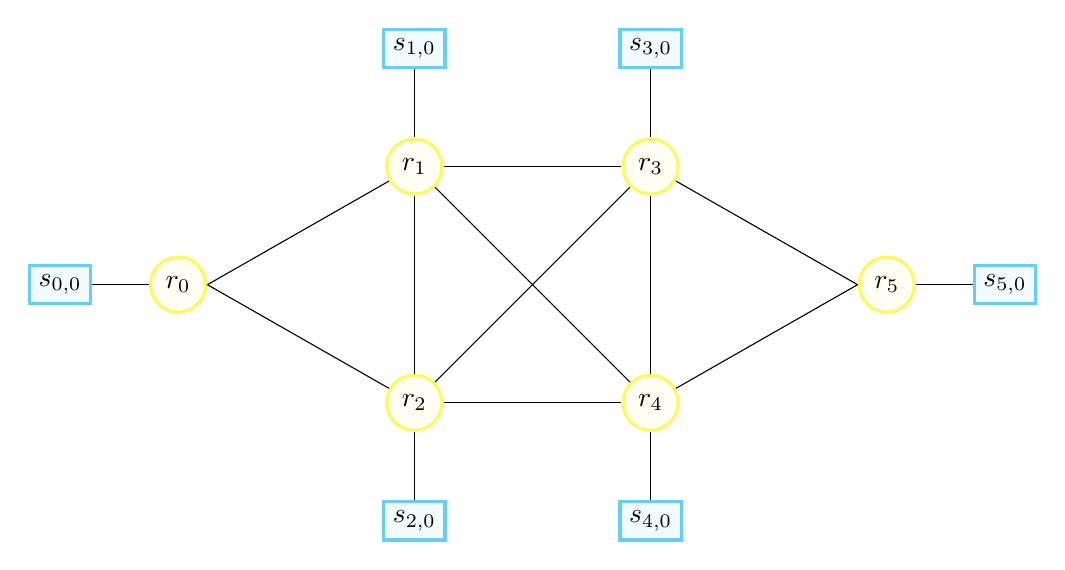
\begin{tikzpicture}[
        router/.style={circle, draw=yellow!60, fill=yellow!5, very thick, minimum size=3.5mm},
        nef_router/.style={circle, draw=red!60, fill=red!5, very thick, minimum size=3.5mm},
        switch/.style={rectangle, draw=cyan!60, fill=cyan!5, very thick, minimum size=2.5mm},
        monitor/.style={rectangle, draw=magenta!60, fill=magenta!5, very thick, minimum size=2.5mm},]
        
        % Routers
        \node[router] (r0) at (-4.5,0)    {$r_0$};
        \node[router] (r1) at (-1.5,1.5)  {$r_1$};
        \node[router] (r2) at (-1.5,-1.5) {$r_2$};
        \node[router] (r3) at (1.5,1.5)   {$r_3$};
        \node[router] (r4) at (1.5,-1.5)  {$r_4$};
        \node[router] (r5) at (4.5,0)     {$r_5$};
        
        %Switches
        \node[switch](s00) at (-6,0)   {$s_{0,0}$};
        \node[switch] (s10) at (-1.5,3)   {$s_{1,0}$};
        \node[switch] (s20) at (-1.5,-3)  {$s_{2,0}$};
        \node[switch] (s30) at (1.5,3)   {$s_{3,0}$};
        \node[switch] (s40) at (1.5,-3)   {$s_{4,0}$};
        \node[switch] (s50) at (6,0)   {$s_{5,0}$};
        %Links
        \draw[-] (r0.east) -- (r1);
        \draw[-] (r0.east) -- (r2);
        \draw[-] (r1) -- (r2);
        \draw[-] (r1) -- (r3);
        \draw[-] (r1.south east) -- (r4.north west);
        \draw[-] (r2) -- (r3);
        \draw[-] (r2) -- (r4);
        \draw[-] (r3) -- (r4);
        \draw[-] (r3) -- (r5.west);
        \draw[-] (r4) -- (r5.west);
        \draw[-] (s00.east) -- (r0.west);
        \draw[-] (s10) -- (r1);
        \draw[-] (s20) -- (r2);
        \draw[-] (s30) -- (r3);
        \draw[-] (s40) -- (r4);
        \draw[-] (s50.west) -- (r5.east);
    \end{tikzpicture}
    \caption[]{Baseline example 6 router network.}
    \label{fig:M6routertop}
\end{figure}

As expected when the nefarious router has a hold probability of 0 it PDV mimics that of a non-nefarious router, however when the nefarious router has a very high hold probability $\gtrapprox 0.7$ we see the PDV regress to that of the rest of the network. We anticipate this behaviour is due to the use of variance as a metric, if a router is delaying all packets traversing it then its queue length will be consistently large or the queue will be completely full, varying little. If this hypothesis is true it follows that although the PDV decreases significantly over a nefarious holding probability of 0.7 the PDA would continue to increase. PDA measurements from the same experimental trials in \ref{fig:MrouterPDA} show a clear monotonic increase between PDA and holding probability, conforming to our expectations.

\sisetup{retain-zero-exponent}
\begin{table}[H]
 \centering
  \begin{tabular}{@{}cS[table-format=1.2e1]@{}}
   \toprule
    \textbf{Hold Probability} & \textbf{Nefarious router} \\
    \textbf{Range} & \textbf{PDA variance} \\
   \midrule
    {[}0.0, 0.1{)} & 3.03e-01  \\
    {[}0.1, 0.2{)} & 8.89e+00  \\
    {[}0.2, 0.3{)} & 1.49e+03  \\
    {[}0.3, 0.4{)} & 9.78e+06  \\
    {[}0.4, 0.5{)} & 8.54e+06  \\
    {[}0.5, 0.6{)} & 6.77e+05  \\
    {[}0.6, 0.7{)} & 1.03e+06  \\
    {[}0.7, 0.8{)} & 2.84e-01  \\
    {[}0.8, 0.9{)} & 3.13e-02  \\
    {[}0.9, 1,0{)} & 3.10e-03  \\
   \bottomrule
  \end{tabular}
  \caption{Variance of nefarious router PDA grouped by varying delay probabilities in the baseline 6 router network.}
    \label{tbl:MrouterPDAvars}
\end{table}
\begin{table}[H]
    \centering
    \aboverulesep = 0pt
    \belowrulesep = 0pt
    \sisetup{table-number-alignment=center}
    \begin{tabular}{l|S[table-format=1.2e1]S[table-format=1.2e1]S[table-format=1.2e1]S[table-format=1.2e1]S[table-format=1.2e1]S[table-format=1.2e1]}
        \toprule
        {\backslashbox{$r_i$}{$r_j$}} & {$r_0$} & {$r_1$} & {$r_2$} & {$r_3$} & {$r_4$} & {$r_5$} \\
        \midrule
        {$r_0$} & 0.0e0  & 5.72e2 & 8.38e2 & 9.90e2 & 6.03e2 & 1.01e2 \\
        {$r_1$} & 5.72e2 & 0.0e0  & 5.58e2 & 7.35e2 & 3.45e1 & 6.37e2 \\
        {$r_2$} & 8.38e2 & 5.58e2 & 0.0e0  & 1.80e2 & 5.74e2 & 9.34e2 \\
        {$r_3$} & 9.90e2 & 7.35e2 & 1.80e2 & 0.0e0  & 7.50e2 & 1.06e3 \\
        {$r_4$} & 6.03e2 & 3.45e1 & 5.74e2 & 7.50e2 & 0.0e0  & 6.67e2 \\
        {$r_5$} & 1.00e2 & 6.37e2 & 9.34e2 & 1.06e3 & 6.67e2 & 0.0e0  \\
        \bottomrule
    \end{tabular}
    \caption{PDA variance between each nefarious router pair $r_i$ and $r_j$}
    \label{tab:Rallvars}
\end{table}
\begin{figure}[H]
    \centering
    \begin{subfigure}{0.475\textwidth}
        \centering
        \includegraphics[width=\textwidth]{figs/results/grouped_summary_avg.png}
        \caption[]{Average Packet Delay}
        \label{fig:MrouterPDA}
    \end{subfigure}
    \begin{subfigure}{0.475\textwidth}
        \centering
        \includegraphics[width=\textwidth]{figs/results/grouped_summary_pdv.png}
        \caption[]{Packet Delay Variation}
        \label{fig:MrouterPDV}
    \end{subfigure}
    \caption{Average non-nefarious and grouped nefarious router packet metrics over a range of time-steps.}
    \label{fig:Rvarnefrouter}
\end{figure}

To investigate if these trends of PDA and PDV hold over arbitrary network topologies 30 random graphs were generated with the ER method, subdivided into 3 groups of 10 graphs each with low ($p=0.2$), medium ($p=0.5$), and high ($p=0.85$) levels of connectivity and 30 were generated with the BA method. Plots of PDV results are shown in \cref{fig:Rrandgraphpdv} with the PDV of the nefarious router shown against the max PDV over all other routers.

\begin{figure}[H]
    \centering
    \missingfigure{Plot of router PDV from rand. graphs}
    \caption{Caption}
    \label{fig:Rrandgraphpdv}
\end{figure}

\subsection{Packet Delay Inference Robustness}
Once again considering the baseline network in \cref{fig:M6routertop} for initial analysis we pivot to examination of the validity of our new inferential method under varied network conditions. The two primary dynamic properties in the simulated network are the length of router queuing buffers and the amount of background traffic which we refer to as traffic intensity. We consider the impact of these properties and their combinatory effects on packet delay metrics.\par

\subsubsection*{Router Queue Buffer Length}
Using the same procedure as baseline experiments in the previous section we consider only the case of $r_1$ begin nefarious, we measure the impact of hold probabilities on packet delay metrics over varying buffer queue lengths. Firstly considering PDA plots of original values and values with a standard min-max normalisation applied are given in \cref{fig:Rvariedqlenpda}.\par
From these we see that irrespective of queue length the relation between hold probability and PDA appears to be a sigmoid curve. Using a standard Levenberg–Marquardt method \cite{osborne_nonlinear_1976} we fit a sigmoid curve of the form $x=a/1+e^{-c\cdot x-d} + b$ to each set of observation results. We selected the Levenberg–Marquardt minimisation algorithm as it performed the best over all fits, both the trust region reflective algorithm and dogleg algorithm with a rectangular trust region were tried but produced inferior $R^2$ values, results for these fits are shown in \cref{Aaltcurvefit}.\par
The fit was calculated to have an $R^2=0.997$ with a minimum of $R^2=0.994$, accurate enough to confirm the initial prediction. In the non-normalised case the upper bound of each sigmoid is given by approximately the maximum length and a lower bound being approximately 0. In normalising the data we see that an increase in queue length both shifts the inflection point of the sigmoid to the right and reduces the gradient of the inflection. The exception to this is queue lengths < 50 where the function seems to behave strangely, we anticipate this is due to the queue easily becoming full, thereafter dropping packets and containing less information, queue lengths this small would however be in practical in real world systems, as such we do not consider these in further analysis and leave them to future work.\par
\begin{figure}[H]
    \centering
    \begin{subfigure}{0.475\textwidth}
        \includegraphics[width=\textwidth]{figs/results/qlen_fitting/qlen_PDA_lm.png}
        \caption{Original}
    \end{subfigure}
    \begin{subfigure}{0.475\textwidth}
        \includegraphics[width=\textwidth]{figs/results/qlen_fitting/norm_qlen_PDA_lm.png}
        \caption{Min-max scaled}
    \end{subfigure}
    \caption{Plots of average nefarious router buffer queue length over various hold probabilities.}
    \label{fig:Rvariedqlenpda}
\end{figure}
To quantify the relationship between queue length and the produced sigmoid we calculate the coefficients for the point of inflection and gradient for each queue length in \cref{fig:Rsigmoidcoefs}. A clear decreasing logarithmic trend can be seen between queue length and inflection point, with an increasing polynomial trend between queue length and inflection gradient. Fitting a polynomial model to this trend we are able to produce a function to estimate the sigmoid curve given a routers queue length. This estimation can allow for the relation to be inverted i.e. given a router's queue length and PDA we can estimate the router's hold probability.
\begin{figure}[H]
    \centering
    \begin{subfigure}{0.475\textwidth}
        \includegraphics[width=\textwidth]{figs/results/qlen_param_c.png}
        \caption{Gradient at inflection point}
    \end{subfigure}
    \begin{subfigure}{0.475\textwidth}
        \includegraphics[width=\textwidth]{figs/results/qlen_param_d.png}
        \caption{X-value of infection point}
    \end{subfigure}
    \caption{Plots of parameters for modeled sigmoid relationship between hold probability and router buffer queue length.}
    \label{fig:Rsigmoidcoefs}
\end{figure}

\subsubsection*{Background Traffic Intensity}

\section{Tomographic Inference}
\begin{figure}[H]
        \centering
        \includegraphics[width=\textwidth]{figs/results/Probe_PDV_accuracy_plot.png}
        \caption{Accuracy of inference from true values over a range of probes sent.}
        \label{fig:Rqstabilization}
\end{figure}
In this section the accuracy of tomographic predictions w.r.t node packet delay metrics are tested.

\subsection{Metric Normalisation}
\label{ssec:Rmetricnormalisation}
The delay distribution and by extension delay variation at a single router is intuitively a combination of the two contributors to \gls{qlen} within the system:
\begin{enumerate}
    \item The \# of packets a router receives.
    \item The \# of packets a router sends.
\end{enumerate}
Contributor \emph{2} is always a fixed rate of 1 packet per time step unless a router is nefarious in which case it will be $<1$ proportional to the router's probability of holding a packet. As the rate of sending is not impacted by contributor \emph{1} we account for variation of contributor \emph{1} between routers to increase the transparency of queuing delay due to variations by contributor \emph{2} within the network.\par
The variation in contributor \emph{1} is proportional to the degree of each node as the number of packets being received by a router each time step is the sum of packets received from each link. Initially we utilized $\sqrt{\gls{routerdeg}}$ for normalization over delay observations by taking $\forall r\in R, \frac{\sigma^2}{\sqrt{\gls{routerdeg}}}$ where $\sigma^2$ is the variance of delay measurements.
\todo{Show results for inferential accuracy RE probing a network where nefarious router has << switches than a non-nef, to demonstrates why we want to normalise for the number of links. }

\section{Optimization Impacts}
\label{sec:Rprobingoptimality}
In this section we apply optimization techniques for selection of monitor nodes, probe paths between these nodes and allocation of probing packets over paths. Inference made under optimized conditions are compared and contrasted to original measures to quantify impact of optimizations, computational costs involved in optimization techniques are weighed against changes in accuracy to assess the practicality of implement these improvements in tomographic monitoring schemes. We begin with monitor placement, extending this with further optimizations with the intent of analyzing the cumulative impact of optimising different aspects of the tomographic pipeline along with individual contributions.
\subsection{Monitor Placement}
\subsection{Path Selection}
\subsection{Probe Allocation}

\section{Real Network Performance}
\label{sec:Rrealnetworkperformance}

\section{Summary}
